\documentclass{article}
\usepackage{graphicx}
\usepackage{amsmath}
\usepackage{comment}
\usepackage{subfigure}
\usepackage[paper=a4paper,%
%            total={14.8cm,22.2cm},%
            top=2.9cm,%
            bottom=3cm,%
            left=1.7cm,%
            right=1.7cm]{geometry}
\linespread{1.3}
\renewcommand{\figurename}{Fig.}
\begin{document}

\begin{center}
  \textbf{\Large Automatic object detection and segmentation from underwater images via saliency-based region merging}\\
  \vskip0.5em
  \textbf{Yafei Zhu$^{1}$}, \textbf{Xinxin Qiu$^{1}$}, \textbf{Xiaoqing Sun$^{1}$}, \textbf{Haiyong Zheng$^{1,\ast}$}, \textbf{Bing Zheng$^{1}$}
  \vskip0.5em
  \bf{1} College of Information Science and Engineering, Ocean University of China, Qingdao, China\\
%  \bf{2} College of Marine Life Science, Ocean University of China, Qingdao, China\\
  $\ast$ E-mail: zhenghaiyong@ouc.edu.cn
\end{center}

Object detection and segmentation from underwater images play an essential role in automatic tracking and recognition of underwater targets such as fishes. Generally, the objects in underwater images are not clearly visible due to low contrast and high noise in the environment, which increases the difficulty of detection and segmentation. Interactive schemes with a few simple user inputs are good solutions for robust detection and accurate segmentation. However, they are usually tedious and not effective in some situations. This paper proposes a novel automatic object detection and segmentation framework to deal with the above problems. Firstly, the dark channel prior~\cite{he2011single} is applied to enhance the image by removing the ``haze'' that makes the underwater image unclear. Then, for detecting salient objects in the enhanced image with complicated background, we choose DRFI~\cite{jiang2013salient} model to generate the saliency map containing ``saliency values'' per pixel. And the obtained saliency map is further processed to determine the location information of object and background. Finally, the region merging based interactive image segmentation method (called MSRM)~\cite{ning2010interactive} is improved by adding the determined object and background information as the user inputs so that the algorithm becomes automatic. The framework of our proposed method is shown in Fig.~\ref{fig:flowchart}. 

%The binary result (Fig.~\ref{fig:flowchart}(f)) shows that our method can extract the salient objects (fishes) from the background effectively.

\begin{figure}[h]
\centerline{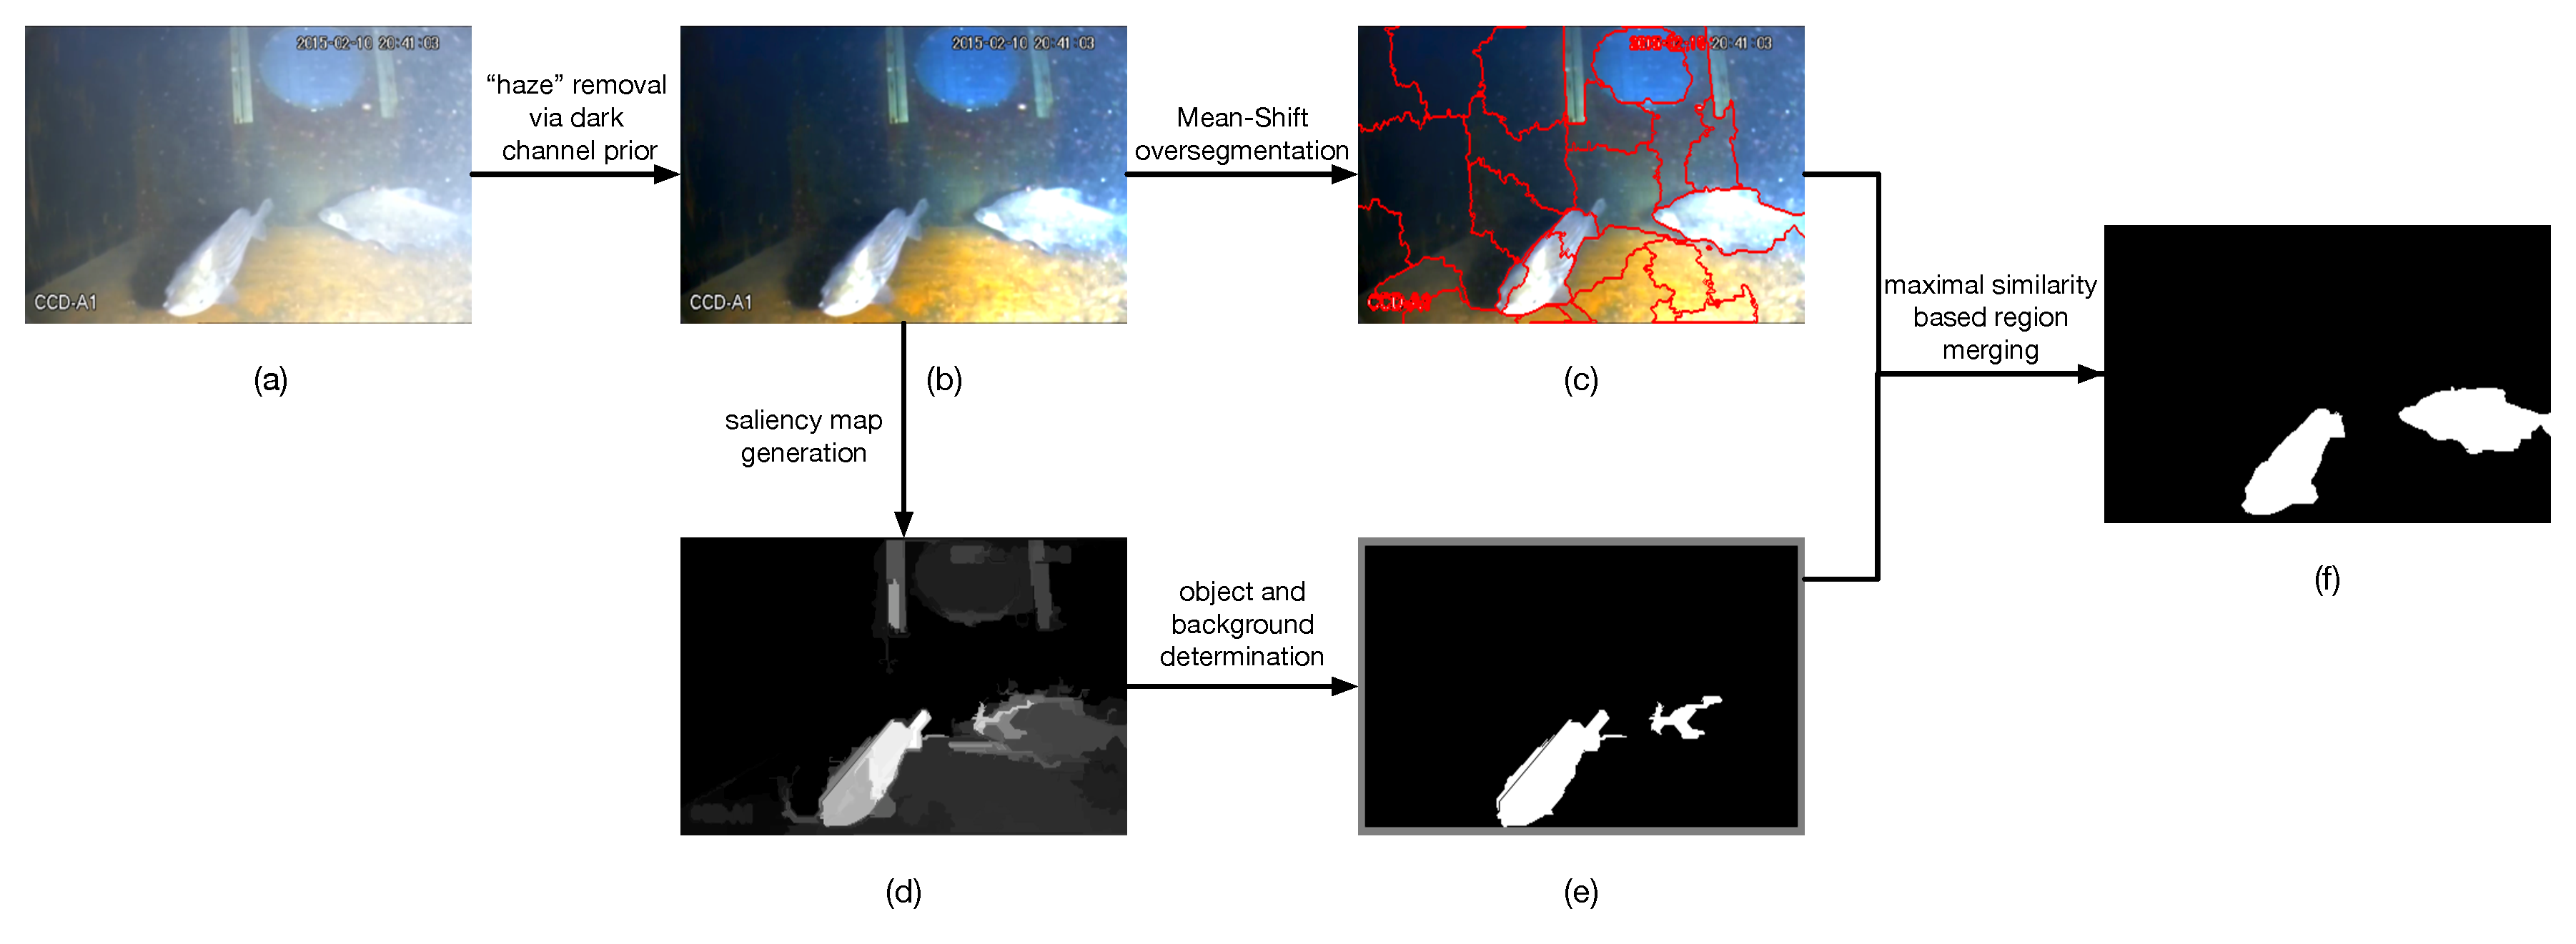
\includegraphics[width=\textwidth]{Figures/flowchart.eps}}
\caption{The framework of our proposed method for object detection and segmentation from underwater images.}
\label{fig:flowchart}
\end{figure} 

The dark channel prior was proposed to remove haze from a single input image~\cite{he2011single}. It is based on the observation that most local patches in haze-free images contain some pixels which have very low intensities in at least one color channel. So dark pixels in the haze image can be used to estimate the haze's transmission and recover the hi-quality haze-free image. The underwater images are similar with the haze images as they are all degraded by medium. The experimental results verify that the dark channel prior can help to enhance the underwater image (Fig.~\ref{fig:flowchart}(b)).

Objects in underwater images may generally draw more attentions of humans at the first sight of the image than the background, hence salient object detection method can be used to approximately obtain the location of the objects, in terms of saliency map. We choose DRFI~\cite{jiang2013salient} to generate the saliency map of enhanced underwater image, since it integrates the regional contrast, regional property and regional backgroundness descriptors together to form the master saliency map, thus can deal with the challenging cases such as detecting salient objects from low-quality underwater images. For each pixel in the saliency map, the higher of the value, the more salient of it in the original image. In other words, normally, for an image, pixels which have higher values in the corresponding saliency map belong to objects. Therefore, pixels whose values in the saliency map are greater than a certain threshold can be taken as object pixels. The Otsu method is adopted to compute the threshold from the saliency map for the determination of object information. We also observed that the image boundary is mostly background, so we take pixels in the $6$-pixel wide narrow border region of the image as background location information. In Fig.~\ref{fig:flowchart}(e), the white parts are the object markers while the gray parts in the image boundary are the background markers, the remaining black parts are non-marked. These markers are used to determine the object and background information automatically instead of user-inputs.

Finally, MSRM~\cite{ning2010interactive} is improved for automatic segmentation by using the extracted object and background information: 
\begin{enumerate}
\item Use Mean-Shift method to generate the oversegmented result (Fig.~\ref{fig:flowchart}(c)) of the enhanced underwater image (Fig.~\ref{fig:flowchart}(b)). 
\item Indicate the initial marker type of each region. For each region in the oversegmented result, we regard it as background, object, or non-marker region using the extracted object and background information respectively.
%we regard it as background region (denoted by $M_B$) if there is at least one background pixel in it, then, a region is regarded as object region (denoted by $M_O$) if the number of object pixels in it accounts for more than 10\% of the region area. If there is neither object nor background pixel in one region, we call it non-marker region, denoted by $N$.
\item Adopt the maximal similarity based region merging mechanism to label all the non-marker regions as either object region or background region recursively so that the objects can be extracted. The similarity between two regions is defined as the Bhattacharyya coefficient of the two corresponding region histogram vectors. If a region $A$ has the maximal similarity (within its neighborhood) with a region $B$, $A$ will be merged to $B$: $B=A\cup B$.

%The color histogram is computed to represent each region, and then . The whole region merging process can be divided into two stages. In the first stage, merging non-marker regions in $N$ with marker background regions in $M_B$. In the second stage, merging non-marker regions in $N$ adaptively.
\end{enumerate}

\begin{figure}[h]
  \centering 
  \subfigure[]{ 
    \label{fig:comparison:a} %% label for first subfigure 
    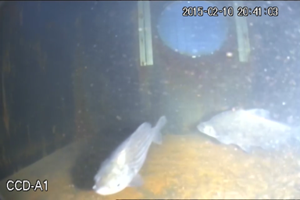
\includegraphics[width=0.25\textwidth]{figures/originalImage.png}} 
  \subfigure[]{ 
    \label{fig:comparison:b} %% label for first subfigure 
    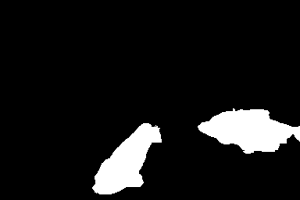
\includegraphics[width=0.25\textwidth]{figures/segmentationResult.png}} 
  \subfigure[]{ 
    \label{fig:comparison:c} %% label for second subfigure 
    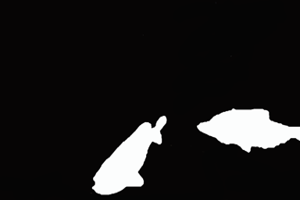
\includegraphics[width=0.25\textwidth]{figures/groundTruth.png}} 
  \caption{Qualitative comparison: (a) Original image. (b) Our segmentation result. (c) Human labeled map.}
  \label{fig:comparison} %% label for entire figure 
\end{figure}

It can be seen from Fig.~\ref{fig:comparison}(b) that it's efficient to segment the salient objects from the underwater image by the proposed method compared with the human labeled ground-truth Fig.~\ref{fig:comparison}(c).
%which can be applied to further procedures such as underwater object tracking and recognition.


\bibliographystyle{plain}

\bibliography{abstract}

\end{document}
